% David Koch

\documentclass[
	headings=optiontotocandhead,% Erweiterung für das optionale Argument der
	% Gliederungsbefehle aktiviert.
	oneside,
	numbers=noenddot,% Keine Punkte am Ende der Gliederungsnummern und davon
	% abgeleiteten Nummern
	toc=flat, %Flache TOC --- kann man anpassen (auskommentieren)
	10pt, % Schriftgröße
	parskip=full, % Abstand zwischen Absätzen (ganze Zeile)
	listof=totoc, % Verzeichnisse im Inhaltsverzeichnis aufführen
	listof=flat, % mehr Abstand für grosse Zahlen
	numbers=noenddot, % kein Punkt am Ende bei Nummern
	%%enlargefirstpage,% Gibt es bei scrartcl nicht!!!!
	bibliography=totoc, % Literaturverzeichnis im Inhaltsverzeichnis aufführen
	%index=totoc, % Index im Inhaltsverzeichnis aufführen
	%captions=tableheading, % Beschriftung von Tabellen für Ausgabe oberhalb
	% der Tabelle formatieren
	%draft % Status des Dokuments (final/draft) draft hinzufügen zum anziegen
	%%der zeilen ende
	a4paper,DIV=14,
	% captions=tablesignature,
]{scrartcl}

\setcounter{secnumdepth}{3}

\usepackage[T1]{fontenc}
\usepackage[utf8]{inputenc}

\usepackage[english, ngerman]{babel, varioref} % your native language must be the last one!!

\usepackage{lastpage}
\usepackage{listings}
\usepackage{blindtext}

%% Aufzählungen nicht so weit einrücken
\usepackage[inline]{enumitem}
%\setitemize{leftmargin=*}
% Listen etwas wenige einrücken, erfordert enumitem
\setitemize{labelindent=2em,labelsep=0.5cm,leftmargin=12ex}

\usepackage{lmodern}

\usepackage{xspace}

\usepackage{graphicx}
\graphicspath{ {../assets} {../assets/Management} }

%%? \usepackage{textcomp}
\usepackage[hyphens]{url}
\usepackage{makeidx}
\makeindex
%%? \usepackage{graphicx}
\usepackage[numbers]{natbib}
\PassOptionsToPackage{normalem}{ulem}
\usepackage{ulem}

\usepackage{needspace}

\setlength\partopsep{0.5ex}%schoenere Listen
\usepackage[bottom]{footmisc}%fussnote ganz unten

\usepackage[]{microtype}
\UseMicrotypeSet[protrusion]{basicmath} % disable protrusion for tt fonts

\usepackage{multirow}   % Allows table elements to span several rows.
\usepackage{booktabs}   % Improves the typesettings of tables.
\usepackage{subcaption} % Allows the use of subfigures and enables their referencing.
\usepackage[ruled,linesnumbered]{algorithm2e} % Enables the writing of pseudo code.
\usepackage[usenames,dvipsnames,table]{xcolor} % Allows the definition and use of colors. This package has to be included before tikz.
\usepackage{nag}       % Issues warnings when best practices in writing LaTeX documents are violated.
\usepackage{todonotes} % Provides tooltip-like todo notes.
\usepackage{placeins}

\usepackage{color}
\usepackage[binary-units]{siunitx}

%% Override default figure placement To be within the flow of the text rather
%% than on it's own page.
% \usepackage{float}
% \makeatletter
% \def\fps@figure{H}
% \makeatother

%% bei vielen Bildern o.ä sinnvoll: Seite muss nicht bis ganz unten gefüllt werden
% \raggedbottom

%\usepackage{footbib} %  footcite, needs other tooling
%% for pandoc2 images
\makeatletter
\def\maxwidth{\ifdim\Gin@nat@width>\linewidth\linewidth\else\Gin@nat@width\fi}
\def\maxheight{\ifdim\Gin@nat@height>\textheight\textheight\else\Gin@nat@height\fi}
\makeatother
% Scale images if necessary, so that they will not overflow the page
% margins by default, and it is still possible to overwrite the defaults
% using explicit options in \includegraphics[width, height, ...]{}
\setkeys{Gin}{width=\maxwidth,height=\maxheight,keepaspectratio}

%% bessere Suche im PDF
\input{glyphtounicode}
\pdfgentounicode=1
%%%%%%%%%%%%%%%%%%%%%%%%%%%%%%%%%%%%%%%%%%%%%%%%%%%%%%%%%%%%%%%%%%%%%%%%%%%%%%%%%%

%  Kopf und Fußzeilen -- links und rechts verschieden
\newcommand{\kopfbild}{\voffset7mm
\includegraphics[width=25mm]{HTL3RLogo}}
\newcommand{\kopfHTL}{\sffamily{\textbf{\large{Projekthandbuch HTL3R}}}}

\usepackage[automark,footsepline,plainfootsepline]{scrlayer-scrpage}
\setkomafont{pageheadfoot}{\normalcolor\footnotesize\scshape}
\setkomafont{pagenumber}{\normalfont\normalsize}
\clearpairofpagestyles
\ihead{\headmark}
\ihead{\kopfbild}
\ohead{\kopfHTL}
\ifoot{\smaller{Höhere Technische Bundeslehranstalt Wien 3 | Rennweg 89b | 1030 Wien | \textcolor{orange}{www.htl.rennweg.at}}}
\ofoot{Seite \pagemark/\pageref{LastPage}}
\ModifyLayer[addvoffset=-.6ex]{scrheadings.foot.above.line}% Linie verschieben
\ModifyLayer[addvoffset=-.6ex]{plain.scrheadings.foot.above.line}% Linie verschieben
\setlength{\headheight}{32pt}

% alle Seiten mit Kopfzeile
%\renewcommand{\chapterpagestyle}{scrheadings}

%% Code Beispiele
%% eine Variante
\usepackage{listings}
\renewcommand{\lstlistingname}{\inputencoding{utf8}Listing}

\usepackage{tabularx}
\usepackage{scrhack}

\usepackage{array}
\newcommand\Tstrut{\rule{0pt}{3.2ex}}         % = `top' strut
\newcommand\Bstrut{\rule[-1.5ex]{0pt}{0pt}}   % = `bottom' strut

\newenvironment{nstabbing}
	{\setlength{\topsep}{-\parskip}
		\setlength{\partopsep}{-\parskip}
		\tabbing}
	{\endtabbing}

\usepackage{titlesec}
% \titleformat{?Überschriftenklasse?}[Absatzformatierung?]{?Textformatierung?} {?Nummerierung?}{?Abstand zwischen Nummerierung und Überschriftentext?}{?Code vor der Überschrift?}[?Code nach der Überschrift?]
\titleformat{\section}[hang]{\Large\bfseries\sffamily}{\thesection\quad}{-1.2ex}{}
\titleformat{\subsection}[hang]{\large\bfseries\sffamily}{\thesubsection\quad}{-1.2ex}{}
\titleformat{\subsubsection}[hang]{\large\bfseries\sffamily}{\thesubsubsection\quad}{-1.2ex}{}
\titleformat{\paragraph}[hang]{\large\bfseries\sffamily}{\theparagraph\quad}{-1.2ex}{}

% \titlespacing{?Überschriftenklasse?}{?Linker Einzug?}{?Platz oberhalb?}{?Platz unterhalb?}[?rechter Einzug?]
\titlespacing{\section}{0pt}{6pt}{6pt}
\titlespacing{\subsection}{0pt}{6pt}{0pt}
\titlespacing{\subsubsection}{0pt}{6pt}{0pt}
\titlespacing{\paragraph}{0pt}{6pt}{0pt}

%% sollte das letzte Package sein
\usepackage[unicode=true,
bookmarks=true,bookmarksnumbered=false,bookmarksopen=false,
breaklinks=true,pdfborder={0 0 0},backref=false,colorlinks=false]
{hyperref}
\hypersetup{pdftitle={Fenrir Management Review vom 12.11.24},
	pdfauthor={Koch, Uhlig, Burger, Vogler},
	pdfsubject={Diplomarbeit},
	pdfkeywords={5CN, DA, Fenrir}}
\urlstyle{same} % don't use monospace font for urls

% Auch Fußnoten bündig ausrichten
\deffootnote[]{1em}{1em}{\textsuperscript{\thefootnotemark\ }}
%% setup
\sloppy % weniger Meldungen
\voffset7mm % etwas nach unten

% \AddToHook{cmd/section/before}{\clearpage}

%%%%%%%%%%%%%%%%%%%%%%%%%%%%%%%%%%%%%%%%%%%%%%%%%%%%%%%%%%%%%%%%%%%%%%%%%%%%%%%%%%
\begin{document}
%% schöner: 10000 -- gar keine, 1000 als Mittelweg
\clubpenalty = 10000 % Schusterjungen verhindern
\widowpenalty = 10000 % Hurenkinder verhindern
\displaywidowpenalty = 1000

{\sffamily{\textbf{\LARGE{\textcolor{orange}{Management Review}}}}}\\
\noindent\rule{\textwidth}{0.1pt}
\begin{nstabbing}
	\hspace{4cm}\=\hspace{4cm}\=\hspace{4cm}\=\kill
	Projekttitel: \> \textbf{Fenrir}\\
	Auftraggeber: \> \textbf{Christian Schöndorfer}\\
	Auftragnehmer: \> \textbf{David Koch}\\
	Schuljahr: \> \textbf{2024/25}
	\> Klasse: \> \textbf{5CN}\\
\end{nstabbing}
{\smaller
	\begin{tabularx}{\textwidth}{l l l l}
	\hline
	\textbf{Version} & \textbf{Datum} & \textbf{Autorin/Autor} & \textbf{Änderung}\Tstrut  \\
	v1.0 & 11.11.2024 & David Koch & Erstellung des Management Reviews\Bstrut  \\
	\hline
	\end{tabularx}
}

\section{Projektstatus}
\textbf{Berichtszeitraum: 08.10.2024 bis 12.11.2024}

Derzeitiger Ampelstatus: Grün

\textbf{Termine}

Alte Rechnung:\\
{\smaller
	\begin{tabularx}{\textwidth}{|X|X|X|X|X|}
		\hline
		\textbf{\% abgeschlossen} & \textbf{Projektstatus} & \textbf{Erwartetes\newline Projektende} & \textbf{Geplantes Projektende} & \textbf{Abweichung} \\
		\hline
		34 & Grün & 14.03.2025 & 14.03.2025 & 0 \\
		\hline
	\end{tabularx}
}
% \% abgeschlossen = Prozentwert, wie viel des Gesamtprojektes abgeschlossen ist. Ermittlung auf der Basis der abgeschlossenen Arbeiten (Stunden) im Verhältnis zu den noch zu erledigenden Arbeiten (in Stunden)

Neue Rechnung:\\
{\smaller
	\begin{tabularx}{\textwidth}{|X|X|X|X|X|}
		\hline
		\textbf{\% abgeschlossen} & \textbf{Projektstatus} & \textbf{Erwartetes\newline Projektende} & \textbf{Geplantes Projektende} & \textbf{Abweichung} \\
		\hline
		58 & Grün & 14.03.2025 & 14.03.2025 & 0 \\
		\hline
	\end{tabularx}
}

\textbf{Kosten}

{\smaller
	\begin{tabularx}{\textwidth}{|X|X|X|X|X|}
		\hline
		\textbf{Ist-Kosten} & \textbf{Restkosten} & \textbf{Erwartete\newline Gesamtkosten} & \textbf{Plankosten} & \textbf{Abweichung} \\
		\hline
		- & - & - & - & - \\
		\hline
	\end{tabularx}
}
% Ist-Kosten = bisher angefallene Kosten in € / bisher angefallene Stunden \\
% Restkosten = welche Kosten bzw. wieviel Stunden sind ab heute bis zum Projektende noch zu erwarten \\
% Erwartete Gesamtkosten = Ist-Kosten + Restkosten bzw. Ist-Aufwand (h) + Restaufwand (h) \\
% Plankosten = ursprünglich (Projektbeginn, Angebot) berechnete Kosten bzw. ursprünglich geschätzter Stundenaufwand \\
% Abweichung = Erwartete Gesamtkosten – Plankosten in € bzw. Erwarteter Gesamtaufwand – Planaufwand (h) \\

\textbf{Stunden}

Alte Rechnung:\\
{\smaller
	\begin{tabularx}{\textwidth}{|X|X|X|X|X|}
		\hline
		\textbf{Ist-Aufwand} & \textbf{Restaufwand} & \textbf{Erwarteter\newline Gesamtaufwand} & \textbf{Planaufwand} & \textbf{Abweichung} \\
		\hline
		407,7 & 790,6 & 1198,3 & 1183 & +15,3 \\ % pfusch
		\hline
	\end{tabularx}
}
% Analog zu den Kosten (siehe oben)

Neue Rechnung:\\
{\smaller
	\begin{tabularx}{\textwidth}{|X|X|X|X|X|}
		\hline
		\textbf{Ist-Aufwand} & \textbf{Restaufwand} & \textbf{Erwarteter\newline Gesamtaufwand} & \textbf{Planaufwand} & \textbf{Abweichung} \\
		\hline
		407,7 & 291,6 & 699,3 & 684 & +15,3 \\ % pfusch
		\hline
	\end{tabularx}
}

\subsection{Teammotivation \colorbox{green!30}{:)}} 
Die Motivation ist im gesamte Team hoch. Die Interesse der Besucher am TOFT und der baldige Besuch der Ukraine-Delegation treibt die Arbeitsmoral voran.

\section{Probleme im Projekt}
Es bestehen derzeit vier bemerkenswerte Probleme im Projekt:
\begin{enumerate}
	\item Die OT-Betriebszelle hätten bereits Anfang November so gut wie fertig sein sollen. Leider ist derzeit jedoch nur Zelle 2 zur Gänze und Zelle 1 zu ca. 60\% fertig aufgebaut, Zelle 3 wurde zu sehr vernachlässigt.
	\item Es fehlen die zwei physischen FortiGate-60F Firewalls, wodurch die Topologie vorerst nicht nach Plan fertiggestellt werden kann.
	\item Die Zeitrechnung der abgeschlossenen Arbeitspakete hat zu wünschen übrig gelassen. In diesem Management Review sind deswegen zwei verschiedene Zeitrechnungen oben inkludiert, jedoch ist die "'neue"' auch nicht perfekt. Die alte Rechnung nimmt alle möglichen Beteiligten eines Arbeitspakets in Betracht, rechnet die für das Arbeitspaket geschätzte Zeit mal der Anzahl der Beteiligten und summiert diese schließlich auf. Die neue Rechnung beschränkt sich im Vergleich zur alten auf eine Person pro Arbeitspaket.
	\item Zeitschätzungen für den Aufbau der OT wurden viel zu optimistisch gewählt. Anstelle von ca. 15h pro Zelle sollten tatsächlich um die 40h geplant gewesen sein $\rightarrow$ lessons learned. Auch die Arbeitspakete hätten granularer definiert werden sollen, um nicht monatelang an einem einzelnen Arbeitspaket (mit 40h Schätzung) zu arbeiten.
\end{enumerate}

\subsection{Problemlösungsstrategie}
So bald es geht zum Kollegen Vogler in den Garten/Keller fahren und alle Zellen fertigstellen. Spätestens bis Ende November sollten alle Zellen in einem brauchbaren Zustand sein und in die HTL Rennweg verlagert werden. Somit können dann permanent die IT- und OT-Netzwerke zusammengeführt werden.

Bezüglich der fehlenden Firewalls und der Zeitrechnungsmethoden sollte Absprache mit den Betreuern gehalten werden.

\subsection{Handlungsbedarf seitens des Managements}
Notwendiger Handlungsbedarf seitens des Managements liegt in folgenden Punkten:

\begin{enumerate}
	\item Das nächste Statusmeeting mit den Betreuern ausmachen
	\item Mögliche Wettbewerbe recherchieren
	\item Kostenaufstellungstabelle vom September ergänzen
\end{enumerate}

\clearpage
\section{Erledigte Arbeiten (vollständig)}
\begin{table}[h]
	\begin{tabularx} {\textwidth} {
			|>{\hsize=.12\hsize}X
			|>{\hsize=.08\hsize}X
			|>{\hsize=.34\hsize}X
			|>{\hsize=.10\hsize}X
			|>{\hsize=.12\hsize}X
			|>{\hsize=.12\hsize}X
			|>{\hsize=.09\hsize}X|
		}
		
		\hline
		\rowcolor[HTML]{D9D9D9} 
		\textbf{\normalsize{Bearbeiter}} & \textbf{\normalsize{PSP-Code}} & {\textbf{\normalsize{Tätigkeit}}} & \textbf{\normalsize{Ort}} & \textbf{\normalsize{Dauer geplant (h)}} & \textbf{\normalsize{Dauer benötigt (h)}} & \textbf{\normalsize{Status}} \\ \hline
		Alle & 1.1.1.1 & Umfang erfassen & - & 8 & ? & \cellcolor{green!30} \\ \hline
		Alle & 1.1.1.2 & Betreuer onboarden & - & 2 & ? & \cellcolor{green!30} \\ \hline
		Alle & 1.1.1.3 & Mögliche Sponsoren/Partner erfassen & - & 4 & ? & \cellcolor{green!30} \\ \hline
		Bastian Uhlig & 1.1.2.1 & Projektidee definieren & - & 3 & 2 & \cellcolor{green!30} \\ \hline
		David Koch & 1.1.2.2 & Provisorische Projektziele definieren & - & 5 & 4,8 & \cellcolor{green!30} \\ \hline
		Gabriel Vogler & 1.1.2.3 & Stakeholder analysieren & - & 4 & 3 & \cellcolor{green!30} \\ \hline
		David Koch & 1.1.2.4 & Risikos analysieren & - & 4 & 4,5 & \cellcolor{green!30} \\ \hline
		Bastian Uhlig & 1.1.2.5 & Spielregeln definieren & - & 5 & ? & \cellcolor{green!30} \\ \hline
		Alle & 1.1.2.6 & Ansuchen schreiben & - & 10 & ? & \cellcolor{green!30} \\ \hline
		Alle & 1.1.2.7 & Antrag schreiben & - & 10 & ? & \cellcolor{green!30} \\ \hline
		David Koch & 1.2.1.1 & OSP erstellen & - & 2 & 1,8 & \cellcolor{green!30} \\ \hline
		David Koch & 1.2.1.2 & PSP erstellen & - & 3 & 3,2 & \cellcolor{green!30} \\ \hline
		Alle & 1.2.1.3 & Arbeitspakete ausdefinieren & - & 12 & ? & \cellcolor{green!30} \\ \hline
		David Koch & 1.3.1.2 & Aufbau \& Funktion der ersten Betriebszelle planen & - & 2 & 1,4 & \cellcolor{green!30} \\ \hline
		David Koch & 1.3.1.2 & Aufbau \& Funktion der zweiten Betriebszelle planen & - & 2 & 7,9 & \cellcolor{green!30} \\ \hline
		Gabriel Vogler & 1.3.1.3 & Aufbau \& Funktion der dritten Betriebszelle planen & - & 2 & 2,8 & \cellcolor{green!30} \\ \hline
		Bastian Uhlig & 1.3.1.5 & SCADA-System planen & - & 8 & 9 & \cellcolor{green!30} \\ \hline
	\end{tabularx}
\end{table}
\FloatBarrier 

\begin{table}[h]
	\begin{tabularx} {\textwidth} {
			|>{\hsize=.12\hsize}X
			|>{\hsize=.08\hsize}X
			|>{\hsize=.34\hsize}X
			|>{\hsize=.10\hsize}X
			|>{\hsize=.12\hsize}X
			|>{\hsize=.12\hsize}X
			|>{\hsize=.09\hsize}X|
		}
		
		\hline
		\rowcolor[HTML]{D9D9D9} 
		\textbf{\normalsize{Bearbeiter}} & \textbf{\normalsize{PSP-Code}} & {\textbf{\normalsize{Tätigkeit}}} & \textbf{\normalsize{Ort}} & \textbf{\normalsize{Dauer geplant (h)}} & \textbf{\normalsize{Dauer benötigt (h)}} & \textbf{\normalsize{Status}} \\ \hline
		Gabriel Vogler & 1.3.2.2 & IT-Server planen & - & 4 & 6,1 & \cellcolor{green!30} \\ \hline
		Julian Burger & 1.3.2.3 & Provisionierung planen & - & 4 & 11 & \cellcolor{green!30} \\ \hline
		David Koch & 1.4.1.5 & OpenPLC SPS programmieren & - & 5 & 1,5 & \cellcolor{green!30} \\ \hline
		Gabriel Vogler & 1.4.1.6 & Siemens LOGO! SPS programmieren & - & 3 & 2 & \cellcolor{green!30} \\ \hline
		Gabriel Vogler & 1.4.2.6 & Windows-Server Provisionierung & - & 30 & 17,5 & \cellcolor{yellow!30} \\ \hline
		Gabriel Vogler & 1.4.2.7 & Windows-Client Provisionierung & - & 10 & 2,5 & \cellcolor{yellow!30} \\ \hline
		Julian Burger & 1.4.2.9 & Provisionierung nach gegebenem Netzplan & - & 15 & 9,25 & \cellcolor{green!30} \\ \hline
		Julian Burger & 1.5.1.1 & Webdesign festlegen & - & 5 & 5,5 & \cellcolor{green!30} \\ \hline
		David Koch & 1.5.1.2 & Randinformationen der technischen Umsetzung festlegen & - & 1 & 1,1 & \cellcolor{green!30} \\ \hline
		David Koch & 1.5.1.3 & easyname kontaktieren & - & 1,5 & 1,25 & \cellcolor{green!30} \\ \hline
		David Koch & 1.5.1.4 & Webinhalte schreiben & - & 3 & 1,4 & \cellcolor{green!30} \\ \hline
		Julian Burger & 1.5.1.5 & Website zusammenfügen & - & 8 & 6 & \cellcolor{green!30} \\ \hline
		David Koch & 1.5.2.1 & Instagram-Konto erstellen & - & 0,5 & 0,4 & \cellcolor{green!30} \\ \hline
		David Koch & 1.5.2.2 & Inhalte für Instagram desginen & - & 3 & 2,75 & \cellcolor{green!30} \\ \hline
		David Koch & 1.5.2.3 & Für das Instagram-Konto werben & - & 5 & 0,75 & \cellcolor{green!30} \\ \hline
		Bastian Uhlig & 1.5.3.1 & Fenrir-Sticker designen & - & 2 & ? & \cellcolor{green!30} \\ \hline
		Bastian Uhlig & 1.5.3.2 & Sticker bestellen & - & 1 & ? & \cellcolor{green!30} \\ \hline
		Bastian Uhlig & 1.5.3.3 & Sticker an Interessierte ausgeben & - & 1 & ? & \cellcolor{green!30} \\ \hline
	\end{tabularx}
\end{table}
\FloatBarrier 

Im Bereich der erledigten Arbeit wurden hauptsächlich Fortschritte im Bereich der OT-Zellen und dessen Steuerungseinheiten, der Einbindung der Nozomi Guardian als auch in der Einbindung des SCADA-Systems gemacht.

Die Arbeitspakete 1.4.2.6 und 1.4.2.7 wurden leicht abgeändert. Der offizielle Bearbeiter ist nun Gabriel Vogler statt Julian Burger, da die Aufsetzung der AD-integrierten Server und Clients in dessen Ziele fällt. Mit einem Bearbeiterwechsel haben sich auch die Arbeitspaketdefinitionen geändert, was dazu führt, dass sie nun auf einem gelben Status gesetzt sind.

\begin{figure}[h]
	\centering
	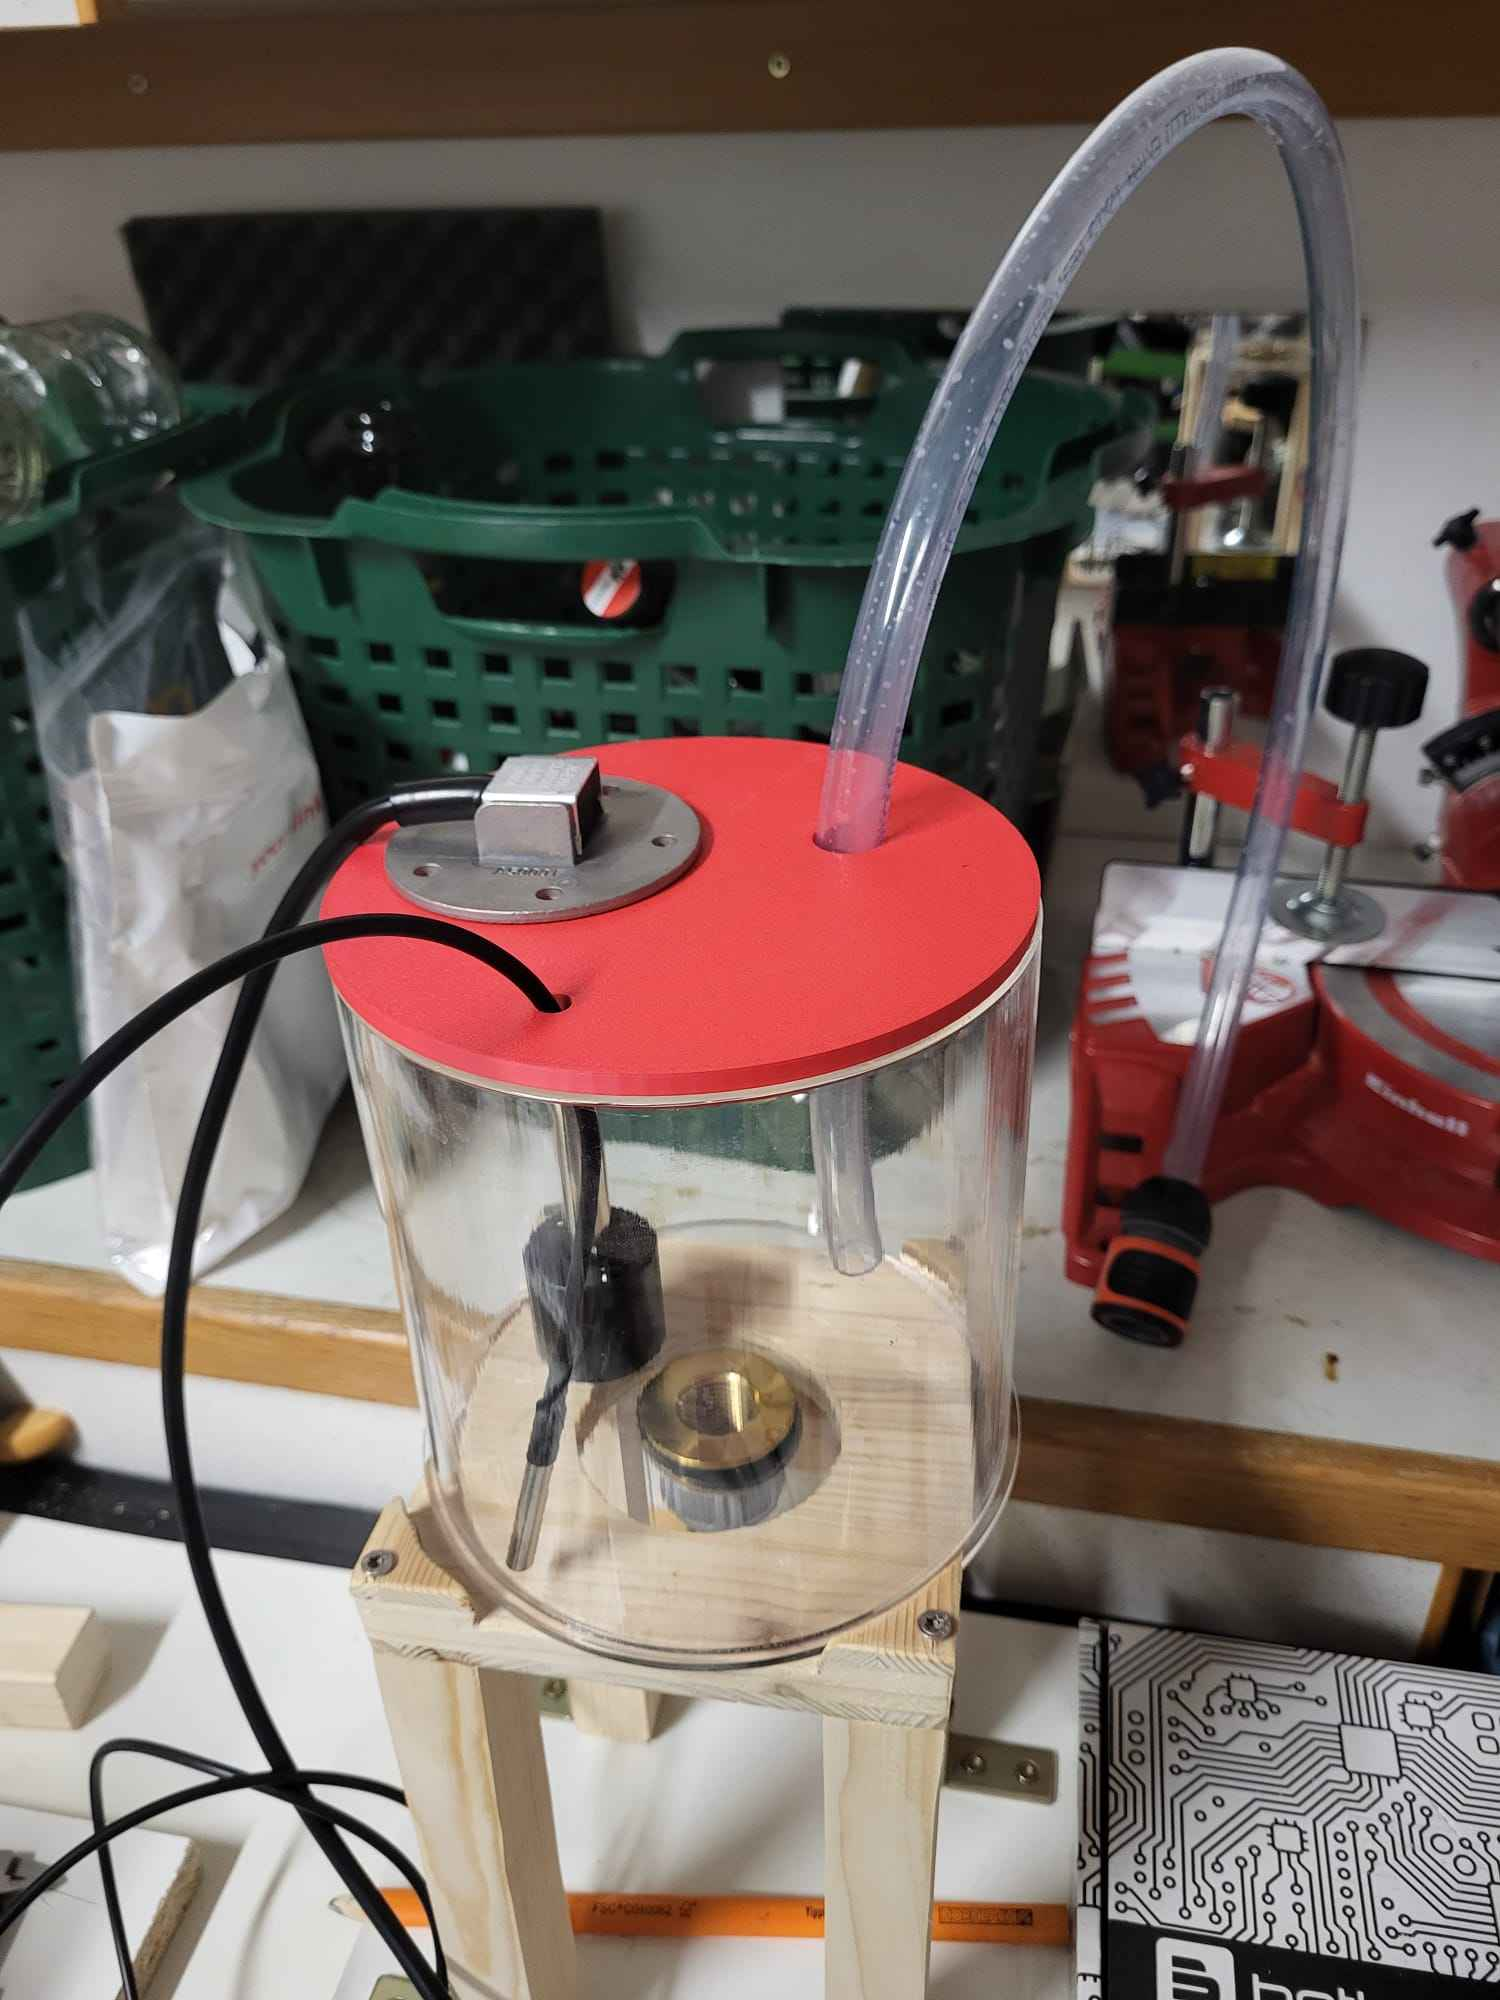
\includegraphics[width=0.9\linewidth]{20241112_1}
	\caption[]{Die fertigen Tanks der ersten Zelle (mit 3D-gedrucktem Deckel)}
\end{figure}
\FloatBarrier 

\begin{figure}[h]
	\centering
	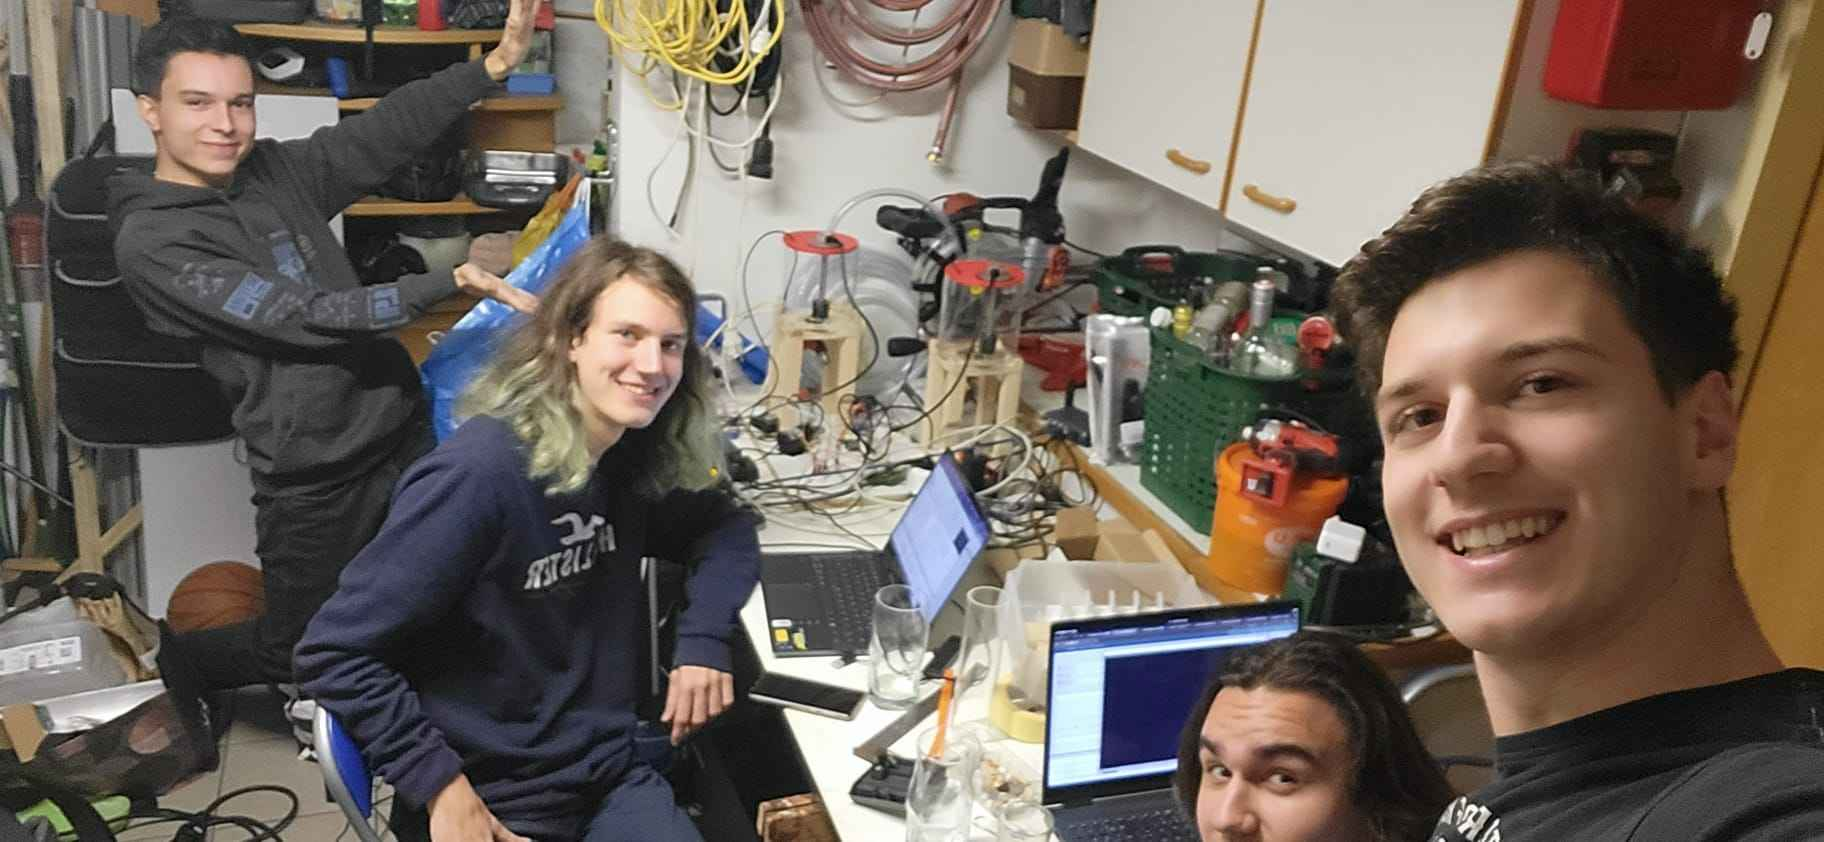
\includegraphics[width=0.9\linewidth]{20241112_2}
	\caption[]{Team Fenrir hart an der Arbeit (Zelle 1 \& 2)}
\end{figure}
\FloatBarrier 

\begin{figure}[h]
	\centering
	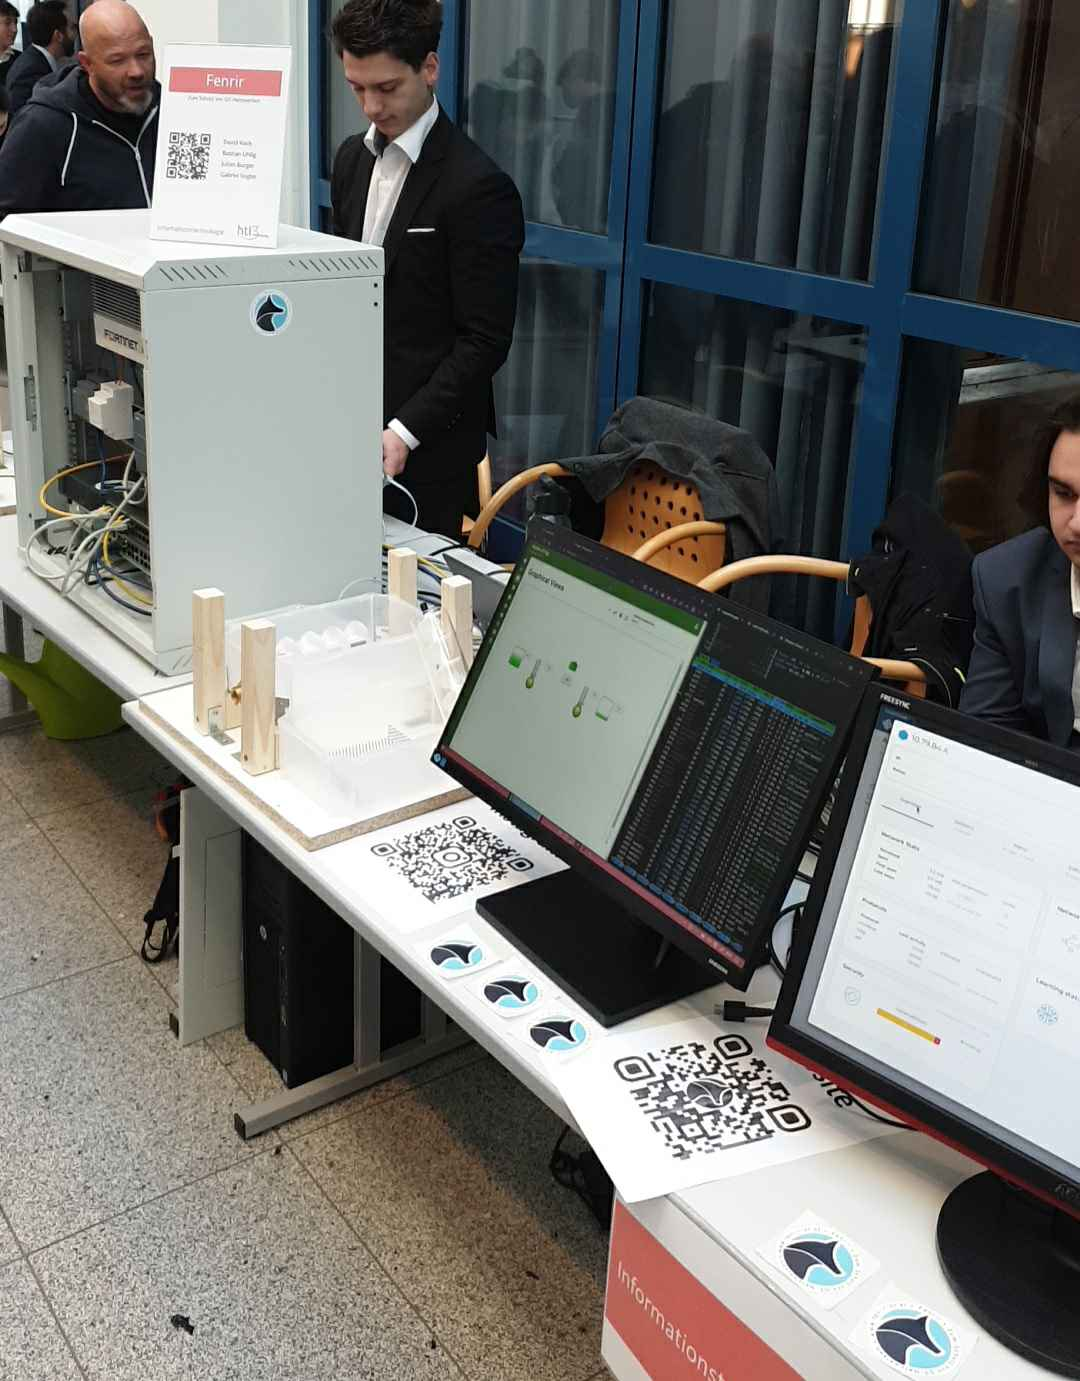
\includegraphics[width=0.9\linewidth]{20241112_3}
	\caption[]{Der Fenrir TOFT-Stand}
\end{figure}
\FloatBarrier 

\clearpage
\section{Anstehende Arbeiten}
\begin{table}[h]
	\begin{tabularx} {\textwidth} {
			|>{\hsize=.12\hsize}X
			|>{\hsize=.08\hsize}X
			|>{\hsize=.54\hsize}X
			|>{\hsize=.12\hsize}X
			|>{\hsize=.15\hsize}X|
		}
		
		\hline
		\rowcolor[HTML]{D9D9D9} 
		\textbf{\normalsize{Bearbeiter}} & \textbf{\normalsize{PSP-Code}} & {\textbf{\normalsize{Tätigkeit}}} & \textbf{\normalsize{Dauer geplant (h)}} & \textbf{\smaller{Fertigstellung geplant}} \\ \hline
		Gabriel Vogler & 1.3.2.1 & AD-Struktur planen & 6 & 20.10.2024 \\ \hline
		David Koch & 1.3.3.3 & Zellen-Firewall-Anforderungen festlegen & 3 & 20.10.2024 \\ \hline
		David Koch & 1.4.1.1 & Erste Betriebszelle aufbauen & 15 & 01.11.2024 \\ \hline
		David Koch & 1.4.1.2 & Zweite Betriebszelle aufbauen & 15 & 01.11.2024 \\ \hline
		Gabriel Vogler & 1.4.1.3 & Dritte Betriebszelle aufbauen & 15 & 01.12.2024 \\ \hline
		David Koch & 1.4.1.4 & Siemens SIMATIC SPS programmieren & 3 & 15.11.2024 \\ \hline
		Bastian Uhlig & 1.4.1.9 & SCADA-System aufgesetzt & 30 & 01.12.2024 \\ \hline
		Julian Burger & 1.4.2.10 & Verifizierung und Überprüfung des automatischen Ablaufes & 10 & 20.10.2024 \\ \hline
		David Koch & 1.4.4.3 & Zellen-Firewall-Konfiguration(en) schreiben & 10 & 15.12.2024 \\ \hline
		Julian Burger & 1.4.4.8 & Jump Server aufgesetzt & 5 & 01.12.2024 \\ \hline
	\end{tabularx}
\end{table}

So bald wie möglich müssen die OT-Betriebszellen fertiggestellt werden. Daraufhin kann die OT und IT das erste miteinander über die geplanten Schnittstellen (FortiGate-Firewalls) kommunizieren, wodurch die ersten Angriffe geplant und ausprobiert werden können. Die Absicherung kann somit voraussichtlich rund um die Weihnachtsferien beginnen.

\end{document}